\documentclass[compress]{beamer}
\usepackage[ngerman]{babel}
\usepackage{graphicx}
\usepackage{subfiles}
\usepackage{listings}

\graphicspath{{images/}}

\setbeameroption{show notes}

\usetheme[noflama]{custom}

\title{Railway-Oriented-Programming \break in Clojure}
\subtitle{Funktionales Error-Handling}
\author{Jan-Philipp Willem}
\institute{Fakultät für Informatik\\Hochschule Mannheim}
\date{EFP, SS2017}

\begin{document}

% \begin{frame}[noframenumbering,plain]
% \end{frame}

% TODO slide background
\maketitle

\begin{frame}[noframenumbering,plain]{Project-Repository}
  \texttt{https://github.com/jwillem/rop-clojure}
\end{frame}

\section*{Gliederung}
\begin{frame}[noframenumbering,plain]{Gliederung}
  \tableofcontents[hideallsubsections]
\end{frame}

\begin{frame}{Scott Wlaschin}
  \setcounter{framenumber}{1}
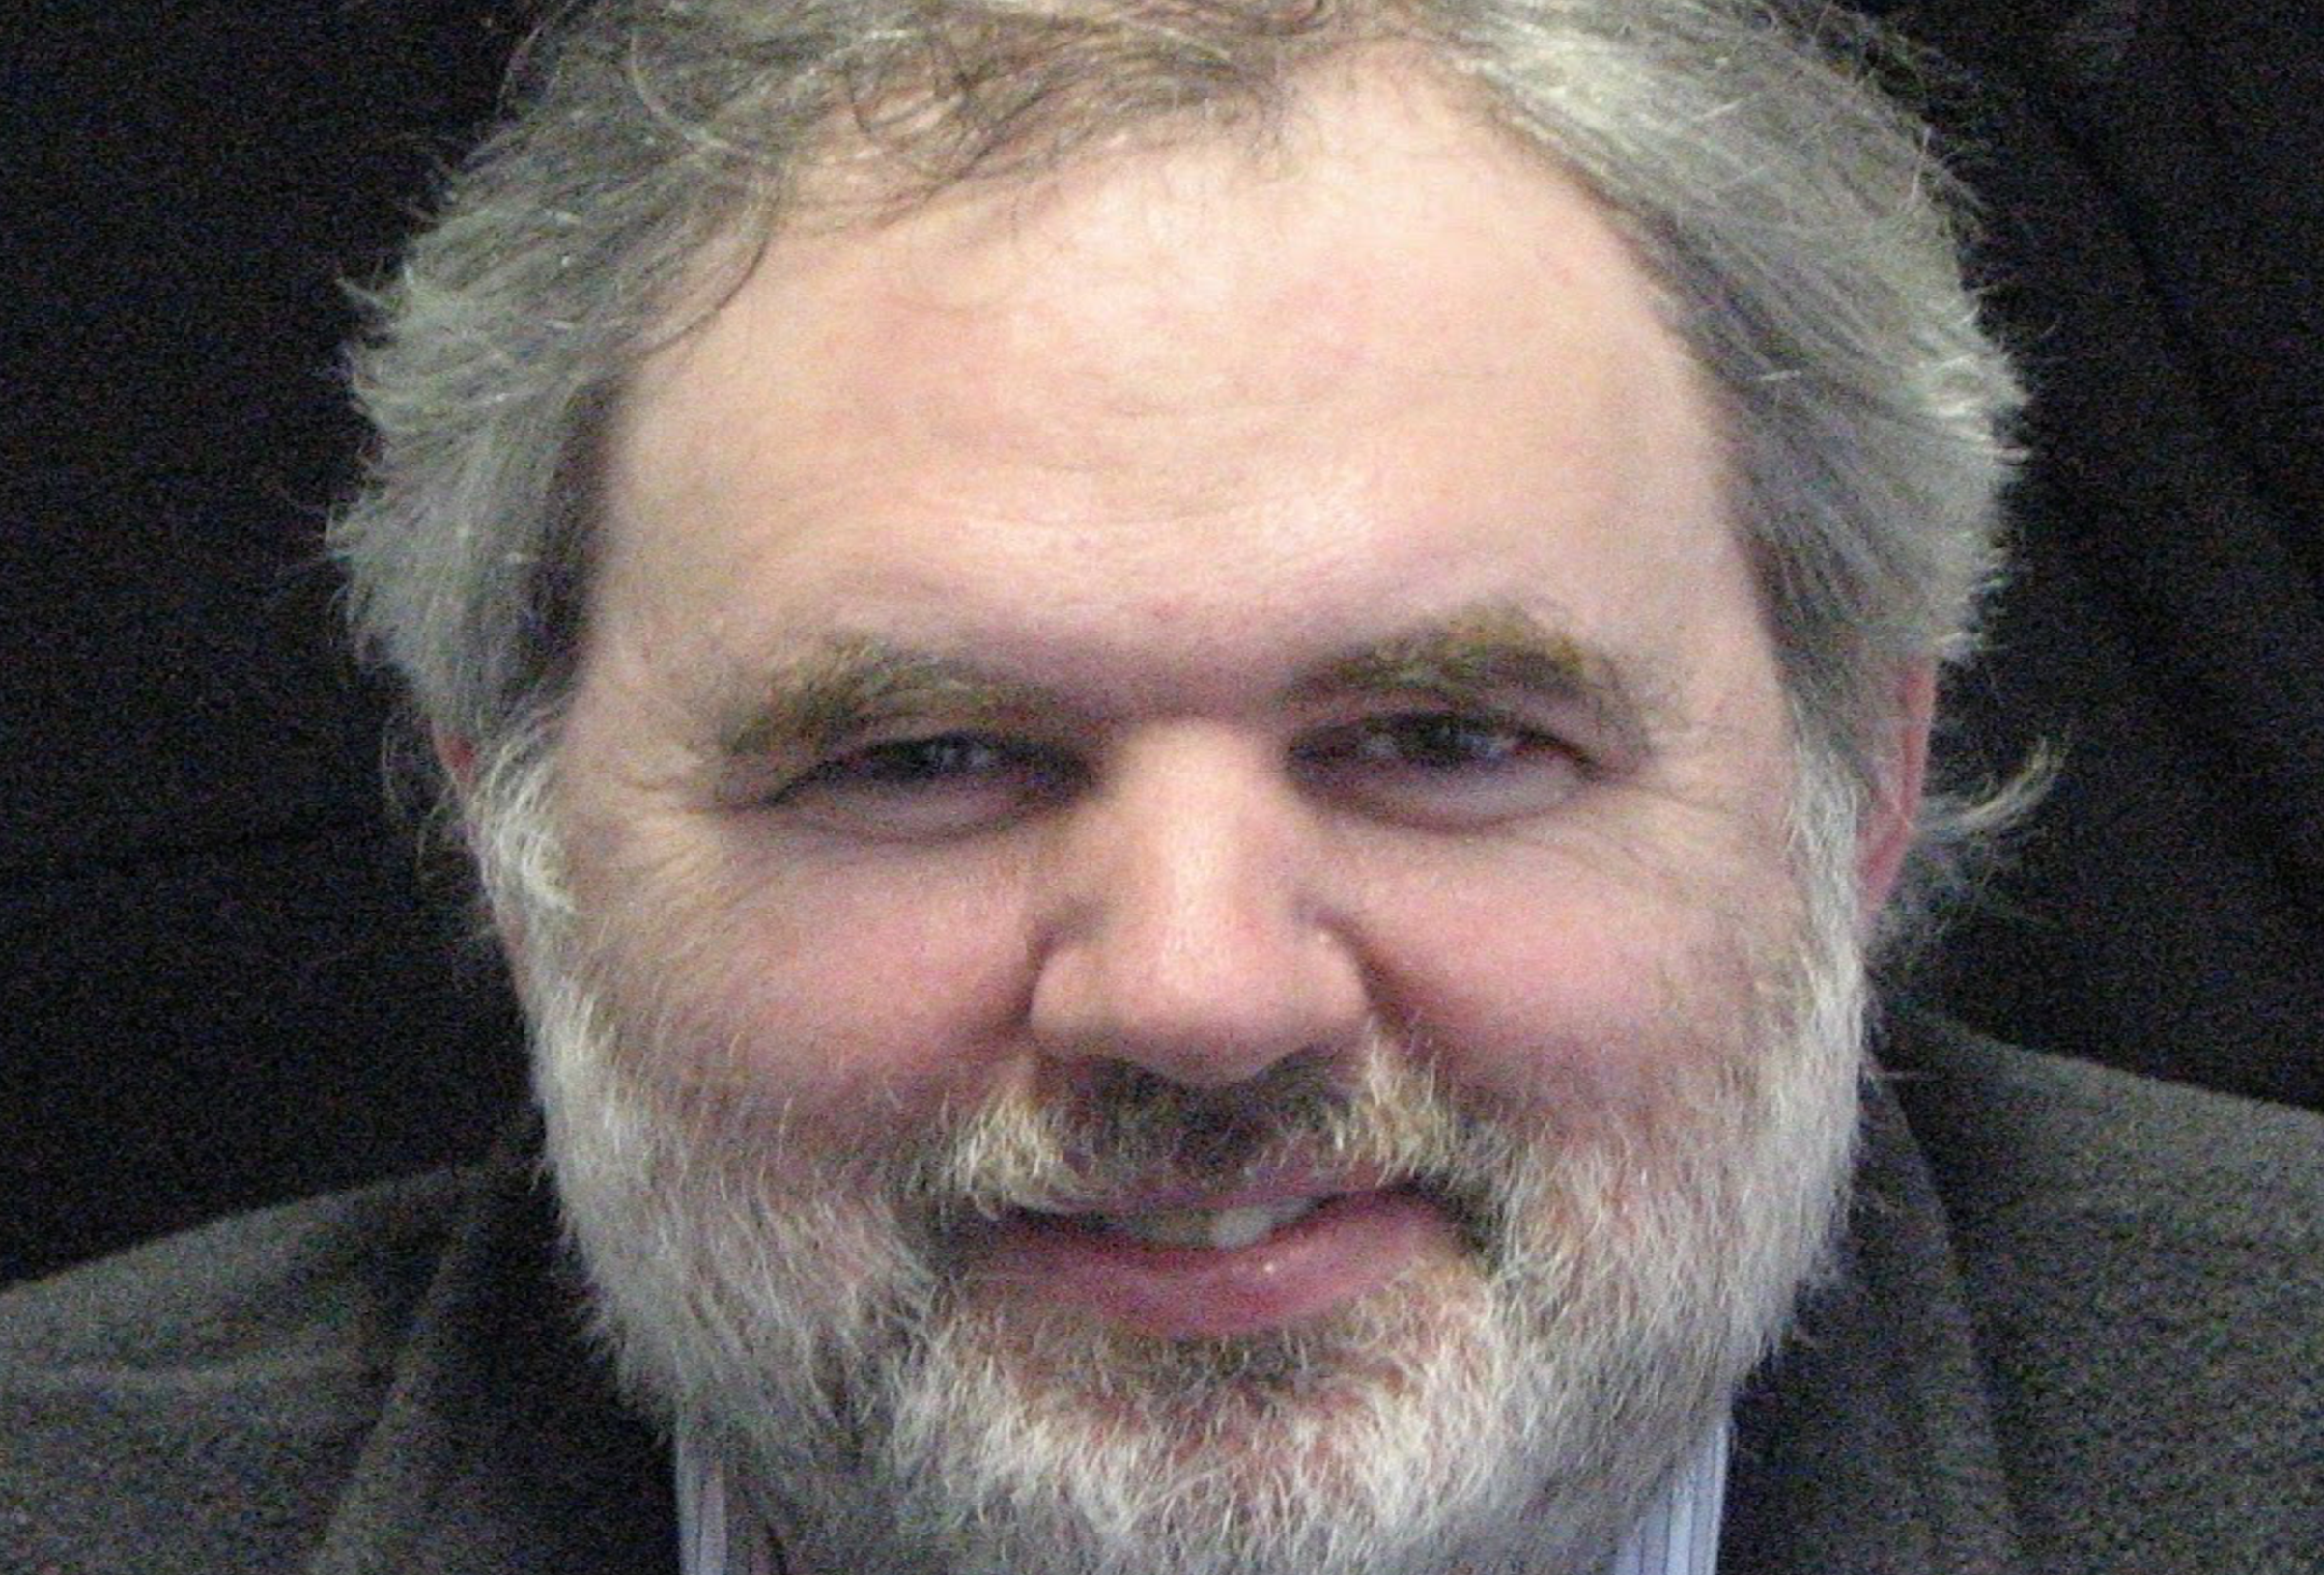
\includegraphics[width=\textwidth]{wlaschin.pdf}
\\[4pt]
https://\textbf{fsharp}forfunandprofit.com/
\end{frame}

% quote as section
\section["`Langes langes Zitat, Lorem Ipsum, weil deswegen und so weiter. Foobar is barbaz and so on."' \small{(Scott Wlaschin, Conference 2015)[1]}]{Who?}

\begin{frame}{Concept}
  \setcounter{framenumber}{3}
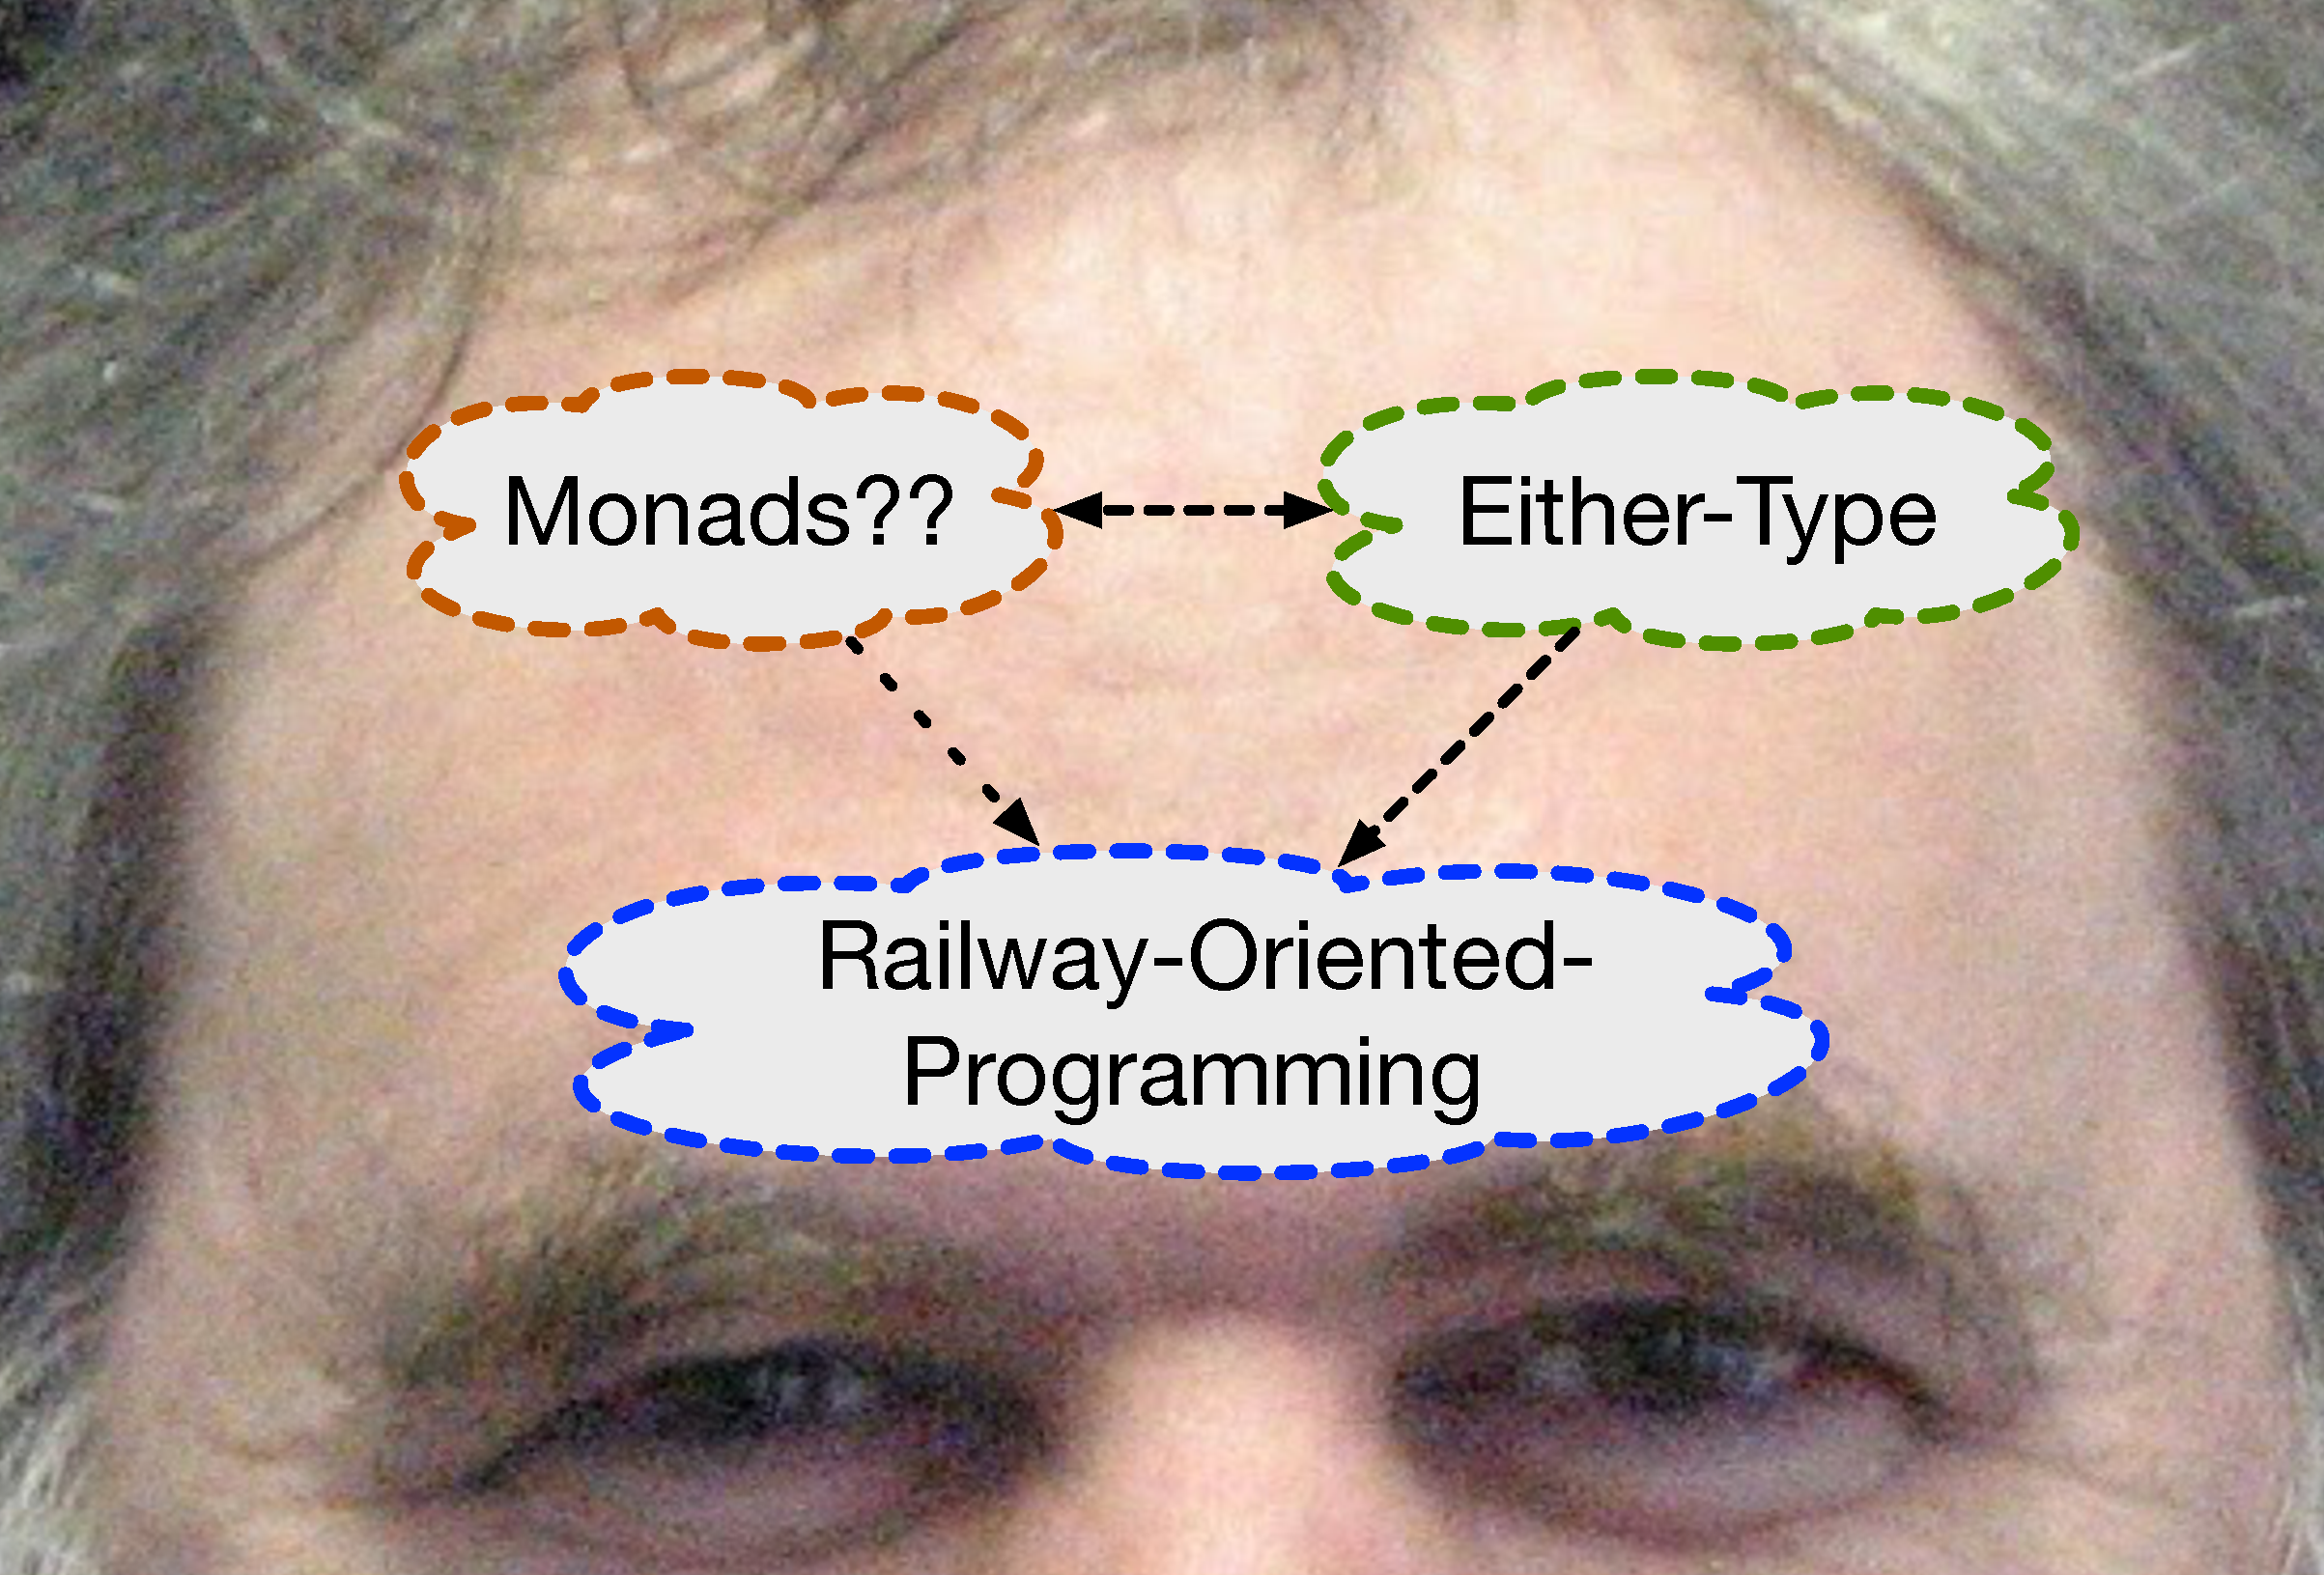
\includegraphics[width=\textwidth]{wlaschin_rop.pdf}
\end{frame}

\section{"`Happy-Path"'}
  \begin{frame}{Usecase: Update Firstname + Email of User (1/2)}
    \begin{columns}[c]
    \column{.6\textwidth}
        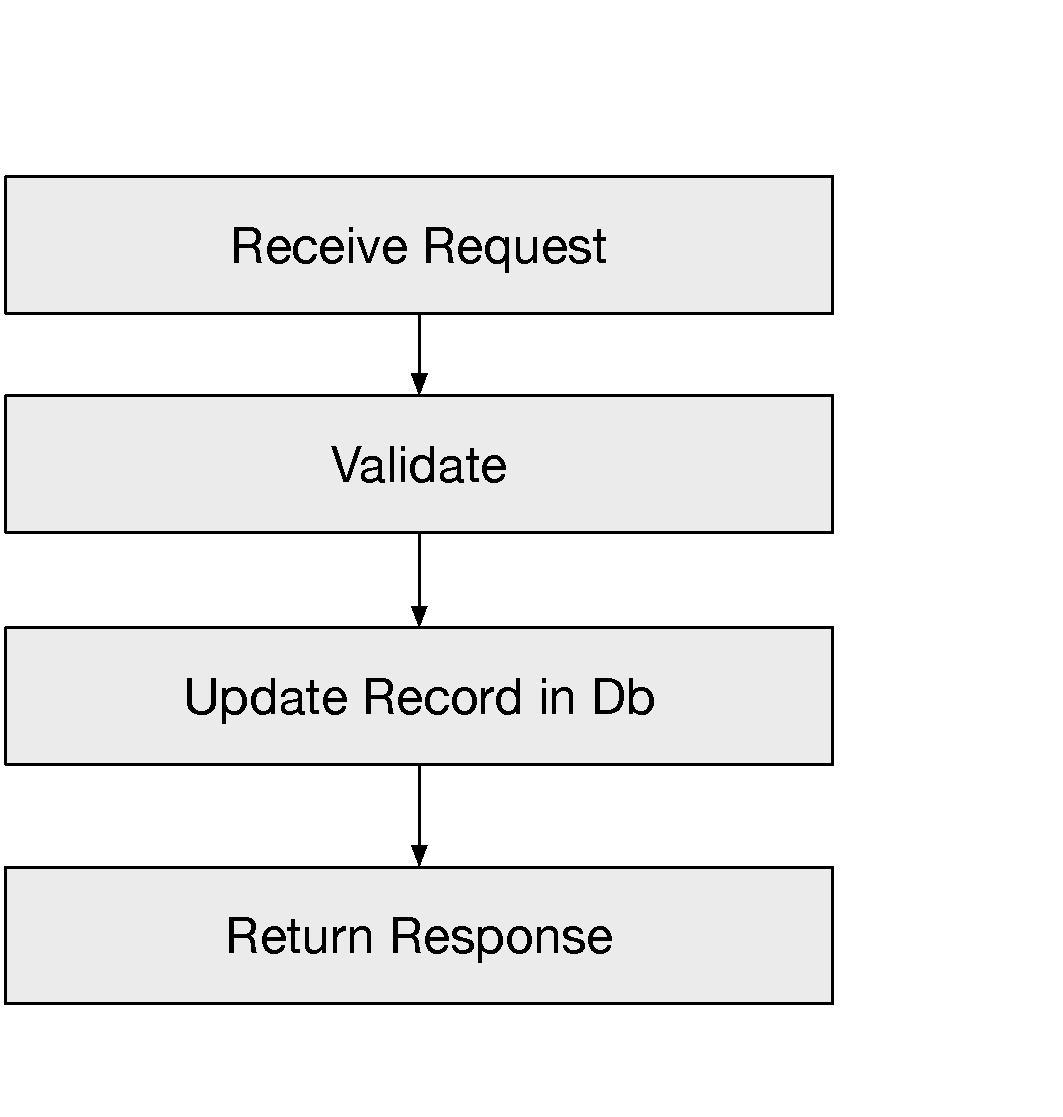
\includegraphics[width=\textwidth]{usecase.pdf}
    \column{.4\textwidth}
    \{\\
      "type": ``user",\\
      "firstname": "Max",\\
      ``email": \\~~~~``max@muster.tld"\\
    \}
    \end{columns}
  \end{frame}
  \begin{frame}{User-Validation mit Node (JS)}
  \end{frame}
  \note[itemize]{%
      \item node-coding-style
  }

\section{Error by design}
  \begin{frame}{Usecase: Update Firstname + Email of User (2/2)}
    \textbf{Und sinnvolle Fehler zurückgeben.}
    \begin{columns}[c]
    \column{.6\textwidth}
    \\ 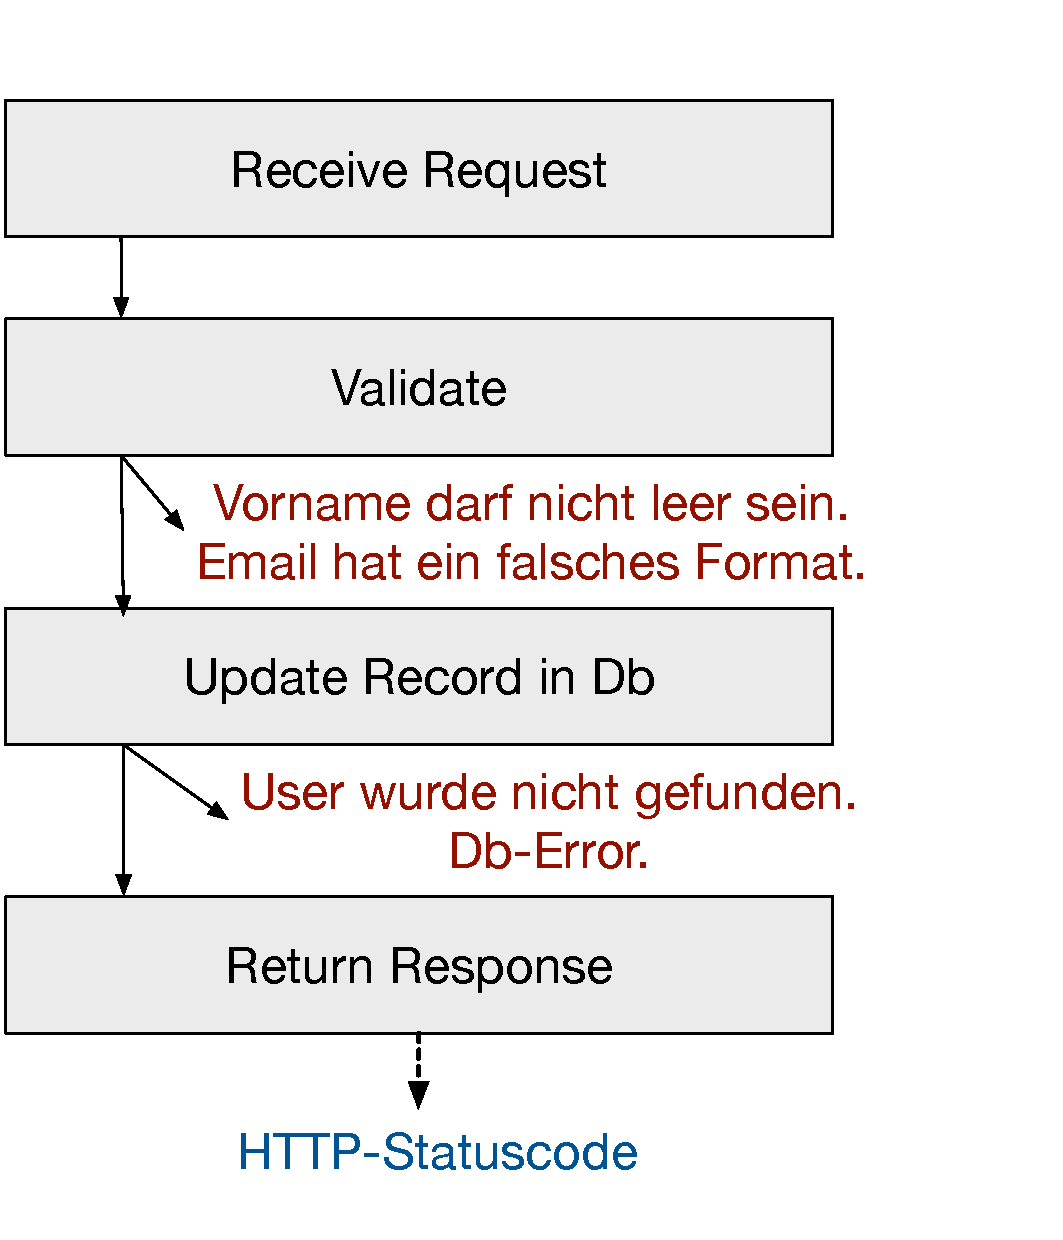
\includegraphics[width=\textwidth]{usecase_error.pdf}
    \column{.4\textwidth}
    \{\\
      "type": ``user",\\
      "firstname": `` `` ,\\
      ``email":\\
      ~~~~``max@@@muster.tld"\\
    \}
    \end{columns}
  \end{frame}
  \begin{frame}{Data-Flow mit Clojure}
     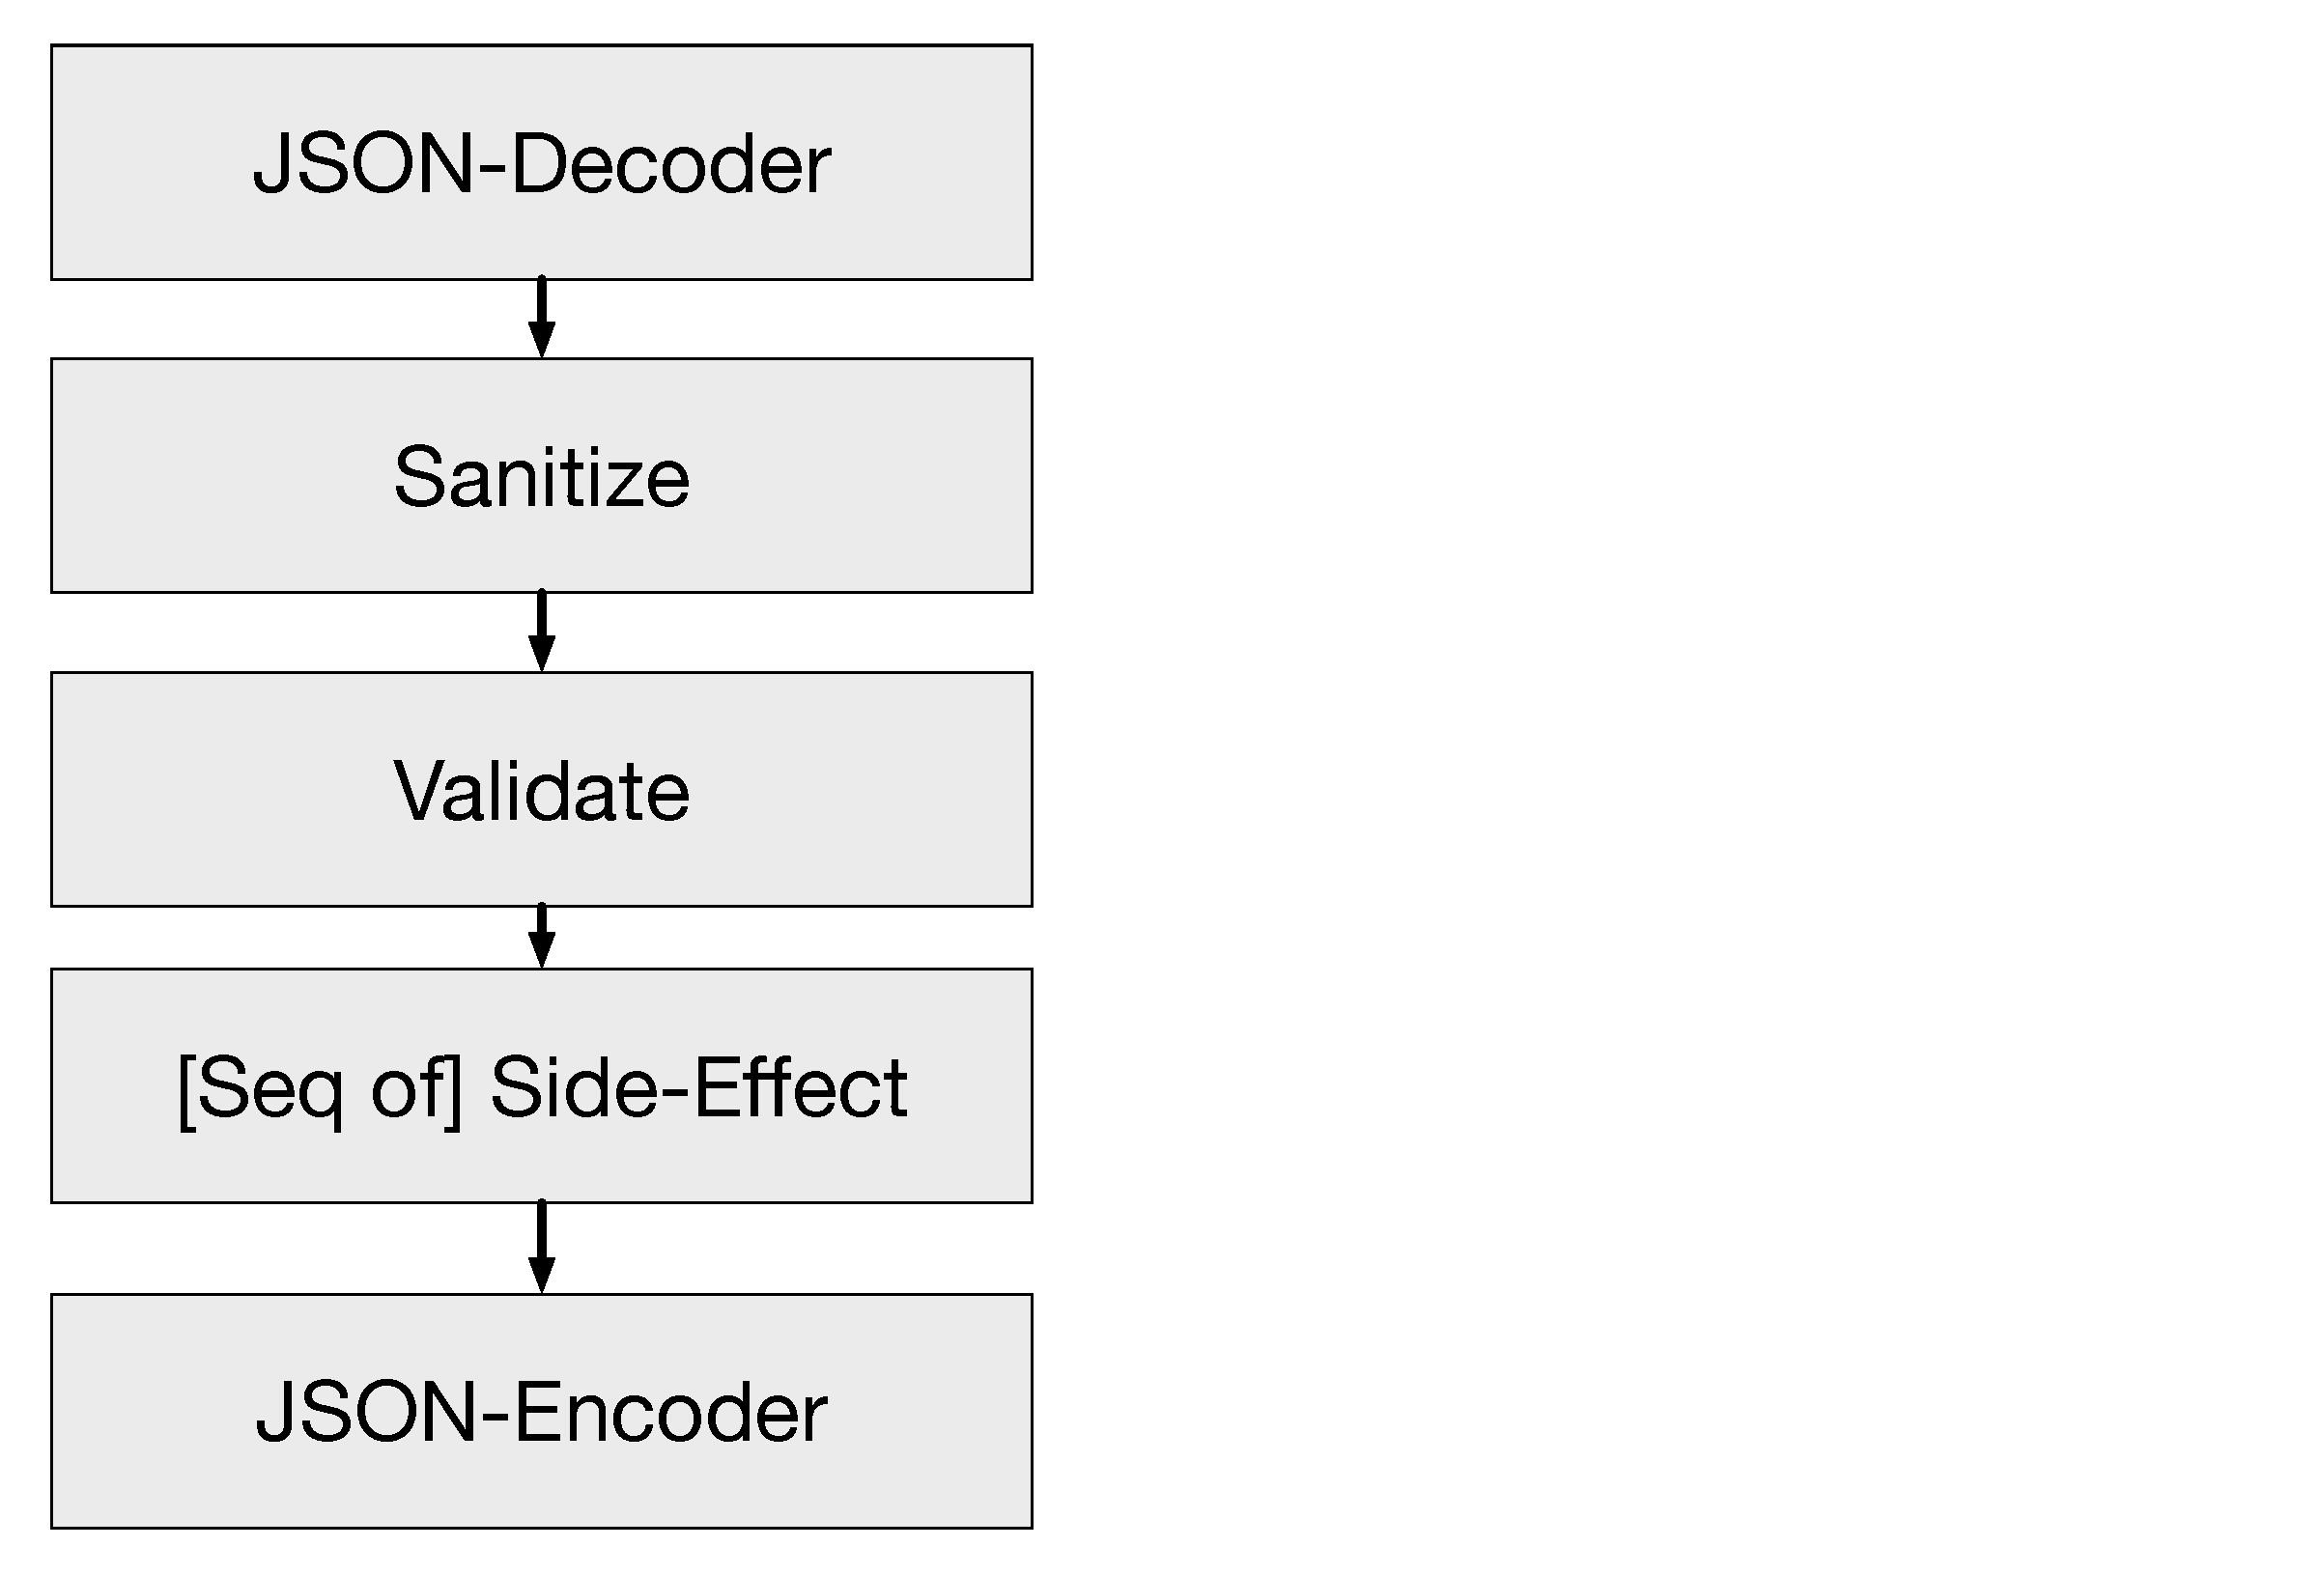
\includegraphics[width=\textwidth]{data_flow.pdf}
  \end{frame}

\section{"`Railway-Oriented-Programming"'}
\begin{frame}{Äpfel \& Birnen}
  \end{frame}
\begin{frame}{Grundlegende Schienenteile}
    \begin{columns}[c]
    \column{.5\textwidth}
      \begin{itemize}
        \item switch-function
        \item<2-> bind
        \item<3-> pipe-bind
        \item<4-> compose
        \item<5-> clojure seq-abstraction
        \item<6-> rest-parameters, \texttt{apply}
      \end{itemize}
    \column{.5\textwidth}
    % \includegraphics[width=\textwidth]{parallel.pdf}
    \end{columns}
  \end{frame}
  \begin{frame}{User-Validation mit ROP}
  \end{frame}

  % \note[itemize]{%
  %     \item 
  % }

  \section{Ausblick}
  \begin{frame}{Weitere Schienenteile}
    \begin{itemize}
      \item try/catch
      \item log
      \item ..
    \end{itemize}
  \end{frame}
  \begin{frame}{Fazit}
  \end{frame}
  
  \begin{frame}[noframenumbering,plain]{Fin}
    Danke für die Aufmerksamkeit. -- Fragen?
  \end{frame}
  \begin{frame}[noframenumbering,plain]{References}
    \begin{itemize}
      \item[1] \texttt{https://vimeo.com/113707214}
      \item[2] \texttt{https://guide.elm-lang.org/error\_handling}
    \end{itemize}
  \end{frame}
\end{document}
